
\begin{theorem}
    Si una recta paralela a un lado de un triángulo, corta a los otros dos lados en puntos distintos, entonces determina sobre ellos segmentos proporcionales.
    
    \begin{figure}[!h]
        \centering
        \input{plots/semejanza/plot600}
        \caption{$DE \parallel BC \imply \dfrac{AB}{AD} = \dfrac{AC}{AE}$}
        \label{fig:parlela-triangular}
    \end{figure}
\end{theorem}

\begin{theorem}[Recíproco del teorema anterior]
    Si una recta interseca dos lados de un triángulo y determina sobre ellos segmentos proporcionales, entonces la recta es paralela al tercer lado.    
\end{theorem}

\begin{theorem}[\textbf{Teorema de Tales}]
    Si tres o más rectas paralelas son intersecadas por dos rectas transversales, los segmentos de las rectas transversales determinados por las rectas paralelas son proporcionales.

    \begin{figure}[!h]
        \centering
        \begin{tikzpicture}

    % Define the points of the transversals
    \tkzDefPoint(0,0){A}
    \tkzDefPoint(8,0){B}
    \tkzDefPoint(1,2){C}
    \tkzDefPoint(7,2){D0}
    \tkzDefPoint(2,4){E}
    \tkzDefPoint(4,4){F}

    \tkzDrawLine[add=0.4 and 0.4,Latex-Latex](E,F)
    \tkzDrawLine[add=0.1 and 0.1,Latex-Latex](A,B)
    
    \tkzDrawLine[add=0.3 and 0.3,Latex-Latex](A,E)
    \tkzDrawLine[add=0.3 and 0.3,Latex-Latex](B,F)
    \tkzDrawLine[add=0.2 and 0.2,dashed,Latex-Latex](A,F)

    \tkzInterLL(C,D)(A,F)
        \tkzGetPoint{H}

    \tkzInterLL(F,B)(C,D0)
        \tkzGetPoint{D}

    \tkzDrawLine[add=0.2 and 0.2,Latex-Latex](C,D)        

    \tkzDrawPoints(A,B,C,D,E,F,H)
    
    \tkzLabelPoint[above left](E){$A$}
    \tkzLabelPoint[above left](C){$B$}
    \tkzLabelPoint[above left](A){$C$}

    \tkzLabelPoint[above right](F){$D$}
    \tkzLabelPoint[above right](D){$E$}
    \tkzLabelPoint[above right](B){$F$}

    \tkzLabelPoint[below right](H){$H$}
    
\end{tikzpicture}
        \caption{$\dfrac{AB}{BC} = \dfrac{DE}{EF} = \dfrac{DH}{HC}$}
        \label{fig:teorema-tales}
    \end{figure}    
\end{theorem}

\clearpage

\begin{definition}[\textbf{Paralela media}]
    El segmento paralelo a uno de los lados de un triángulo y que contiene los puntos medios de los otros dos lados, recibe el nombre de \textit{paralela media}.
\end{definition}

\begin{theorem}[\textbf{Paralela media es mitad de la base}]
    El segmento que interseca dos lados de un triángulo en sus puntos medios es paralelo al tercer lado y mide la mitad de este.
\end{theorem}

\begin{figure}[!h]
    \centering
    \input{plots/semejanza/plot602}
    \caption{Paralela media: $DE = \dfrac{1}{2}BC$}
    \label{fig:paralela-media}
\end{figure}    

\subsection{Triángulos Semejantes}

\begin{definition}[\textbf{Triángulos semejantes}]
    Dada una correspondencia entre dos triángulos, estos son \textit{semejantes} si cumplen que:

    \begin{itemize}
        \item Sus lados correspondientes son proporcionales.
        \item Sus ángulos correspondientes son congruentes.
    \end{itemize}
    
\end{definition}

\begin{definition}[\textbf{Razón de semejanza}]
    La \textit{razón de semejanza} es el cociente de las medidas de los dos lados correspondientes en triángulos semejantes.
\end{definition}


\subsection{Teoremas de Semejanza Triangular}

\begin{theorem}[\textbf{Ángulo,Ángulo,Ángulo: a-a-a}]
    Dada una correspondencia entre dos triángulos, si los tres pares de ángulos correspondientes son congruentes entonces los triángulos son semejantes.
\end{theorem}


\begin{theorem}[\textbf{Ángulo,Ángulo: a-a}]
    Dada una correspondencia entre dos triángulos, si dos pares de ángulos correspondientes son congruentes entonces los triángulos son semejantes.
\end{theorem}


\begin{theorem}[\textbf{Lado,Ángulo,Lado: l-a-l}]
    Dada una correspondencia entre dos triángulos, si dos pares de lados correspondientes son proporcionales y el ángulo comprendido entre ellos es congruente, entonces los triángulos son semejantes.
\end{theorem}

\begin{theorem}[\textbf{Lado,Lado,Lado: l-l-l}]
    Dada una correspondencia entre dos triángulos, si los tres pares de lados correspondientes son proporcionales, entonces los triángulos son semejantes.
\end{theorem}

\subsection{Semejanza de Polígonos}

\begin{definition}[\textbf{Polígonos semejantes}]
    Dos \textit{polígonos} son \textit{semejantes} si sus ángulos correspondientes son congruentes y sus lados correspondientes son proporcionales.
\end{definition}


\subsection{Teorema de Pitágoras}

\begin{theorem}[\textbf{Pitágoras}]
    En todo triángulo rectángulo, el cuadrado de la longitud de la hipotenusa es igual a la suma de los cuadrados de las longitudes de los catetos.
\end{theorem}

\begin{theorem}[\textbf{Recíproco de Pitágoras}]
    Si el cuadrado de la longitud de un lado de un triángulo es igual a la suma de los cuadrados de las longitudes de los otros dos lados, entonces el triángulo es rectángulo, con su ángulo recto opuesto al lado de mayor longitud.
\end{theorem}

\begin{definition}[\textbf{Proyección de la altura sobre la hipotenusa en un triángulo rectángulo}]

    La altura sobre la hipotenusa de un triángulo rectángulo divide a la hipotenusa en dos segmentos llamados \textit{proyecciones} de cada uno de los catetos del triángulo sobre la hipotenusa.

    \begin{figure}[!h]
        \centering
        \input{plots/semejanza/plot603}
        \caption{Proyección de la altura sobre la hipotenusa}
        \label{fig:proyec-altura-hipotenusa}
    \end{figure}    

    En la figura, $h$ es la altura sobre la hipotenusa que divide a $c$ en dos segmentos $m$ y $n$ en donde $m$ es la proyección del cateto $\seg{AC}$ sobre la hipotenusa y $n$ es la proyección del cateto $\seg{BC}$ sobre la hipotenusa.
\end{definition}

\clearpage

\begin{theorem}[\textbf{altura sobre la hipotenusa de un triángulo rectángulo}]
    El cuadrado de la medida de la altura sobre la hipotenusa en un triángulo rectángulo es igual al producto de la longitud de las proyecciones de los catetos sobre la hipotenusa.

    \begin{figure}[!h]
        \centering
        \input{plots/semejanza/plot603}
        \caption{$h^2 = m \cdot n$}
        \label{fig:projection-hipotenusa-cateto}
    \end{figure}    
    
\end{theorem}

\begin{theorem}[\textbf{Del cateto}]
    El cuadrado de la longitud de un cateto es igual al producto de la longitud de la proyección de dicho cateto sobre la hipotenusa por la longitud de la hipotenusa.

    \begin{figure}[!h]
        \centering
        \input{plots/semejanza/plot604}
        \caption{$b^2 = m \cdot c$ y $a^2 = n \cdot c$}
        \label{fig:proyec-hipotenusa-producto}
    \end{figure}    
    
\end{theorem}

\clearpage

\subsubsection{Triángulos Especiales}

\begin{theorem}[\textbf{Hipotenusa de triángulo rectángulo isósceles}]

    En un triángulo rectángulo isósceles, la medida de la hipotenusa es $\sqrt{2}$ veces mayor que la medida de un cateto.

    \begin{center}
        \noindent 
        \begin{minipage}{0.2\textwidth}
            \vspace{0.5cm}
            \centering
            \begin{tikzpicture}[xscale=-1]
    % Define points for the triangles
    \tkzDefPoint(0,4){A}
    \tkzDefPoint(0,0){B}
    \tkzDefPoint(4,0){C}

    \tkzDrawPolygon(A,B,C)

    \tkzLabelSegment[right](A,B){$a$}
    \tkzLabelSegment[below](B,C){$a$}
    \tkzLabelSegment[above left](A,C){$x$}

    \tkzMarkAngle[arc=l,size=0.8](B,A,C)
    \tkzMarkAngle[arc=l,size=0.8](A,C,B)

    \tkzMarkRightAngle(A,B,C)


\end{tikzpicture}
            \label{fig:rectangulo-isosceles}
        \end{minipage}
        \hspace{0.01\textwidth}
        \begin{minipage}{0.4\textwidth}
            \begin{equation*}
                \begin{split}
                    x^2 &= a^2 + a^2 \\
                    x^2 &= 2a^2 \\
                    x &= \sqrt{2a^2} \\
                    x &= a\sqrt{2}
                \end{split}
            \end{equation*}
        \end{minipage}
    \end{center}
\end{theorem}

\begin{theorem}[\textbf{Cateto mayor de triángulo semi-equilátero}]
    En un triángulo rectángulo semi-equilátero, el cateto mayor mide $\frac{\sqrt{3}}{2}$ veces la medida de la hipotenusa.

    \begin{center}
        \noindent
        \begin{minipage}{0.3\textwidth}
            \vspace{0.5cm}
            \begin{tikzpicture}
    % Definir los puntos del triángulo equilátero
    \tkzDefPoint(0,0){A}
    \tkzDefShiftPoint[A](60:5){B}
    \tkzDefShiftPoint[A](0:5){C}
    
    % Dibujar el triángulo
    \tkzDrawPolygon(A,B,C)

    % Calcular el ortocentro (intersección de las alturas)
    \tkzDefMidPoint(A,C)
    \tkzGetPoint{H}
    \tkzDrawSegment[dashed](B,H)

    \tkzLabelSegment[above left](A,B){$a$}
    \tkzLabelSegment[above right](B,C){$a$}
    \tkzLabelSegment[right](B,H){$h$}
    \tkzLabelSegment[below](A,H){$\frac{a}{2}$}
    \tkzLabelSegment[below](H,C){$\frac{a}{2}$}

    \tkzMarkRightAngle(B,H,A)
    \tkzMarkRightAngle(B,H,C)

    \tkzMarkAngle[arc=l,size=0.8](A,B,C)
    \tkzMarkAngle[arc=l,size=0.8](B,C,A)
    \tkzMarkAngle[arc=l,size=0.8](C,A,B)
    
\end{tikzpicture}
            \label{fig:triángulo semi-equilatero}
        \end{minipage}
        \hspace{0.05\textwidth}
        \begin{minipage}{0.3\textwidth}
            \begin{equation*}
                \begin{split}
                    a^2 &=  \left(\dfrac{a}{2}\right)^2 + h^2 \\
                    h^2 &= a^2 - \dfrac{a^2}{4} \\
                    h^2 &= \dfrac{3a^2}{4}  \\
                    h &= a\dfrac{\sqrt{3}}{2}
                \end{split}
            \end{equation*}
        \end{minipage}
        \hspace{0.05\textwidth}
    \end{center}
    
\end{theorem}

